%%pull out cause not helping
\begin{figure}[H]
    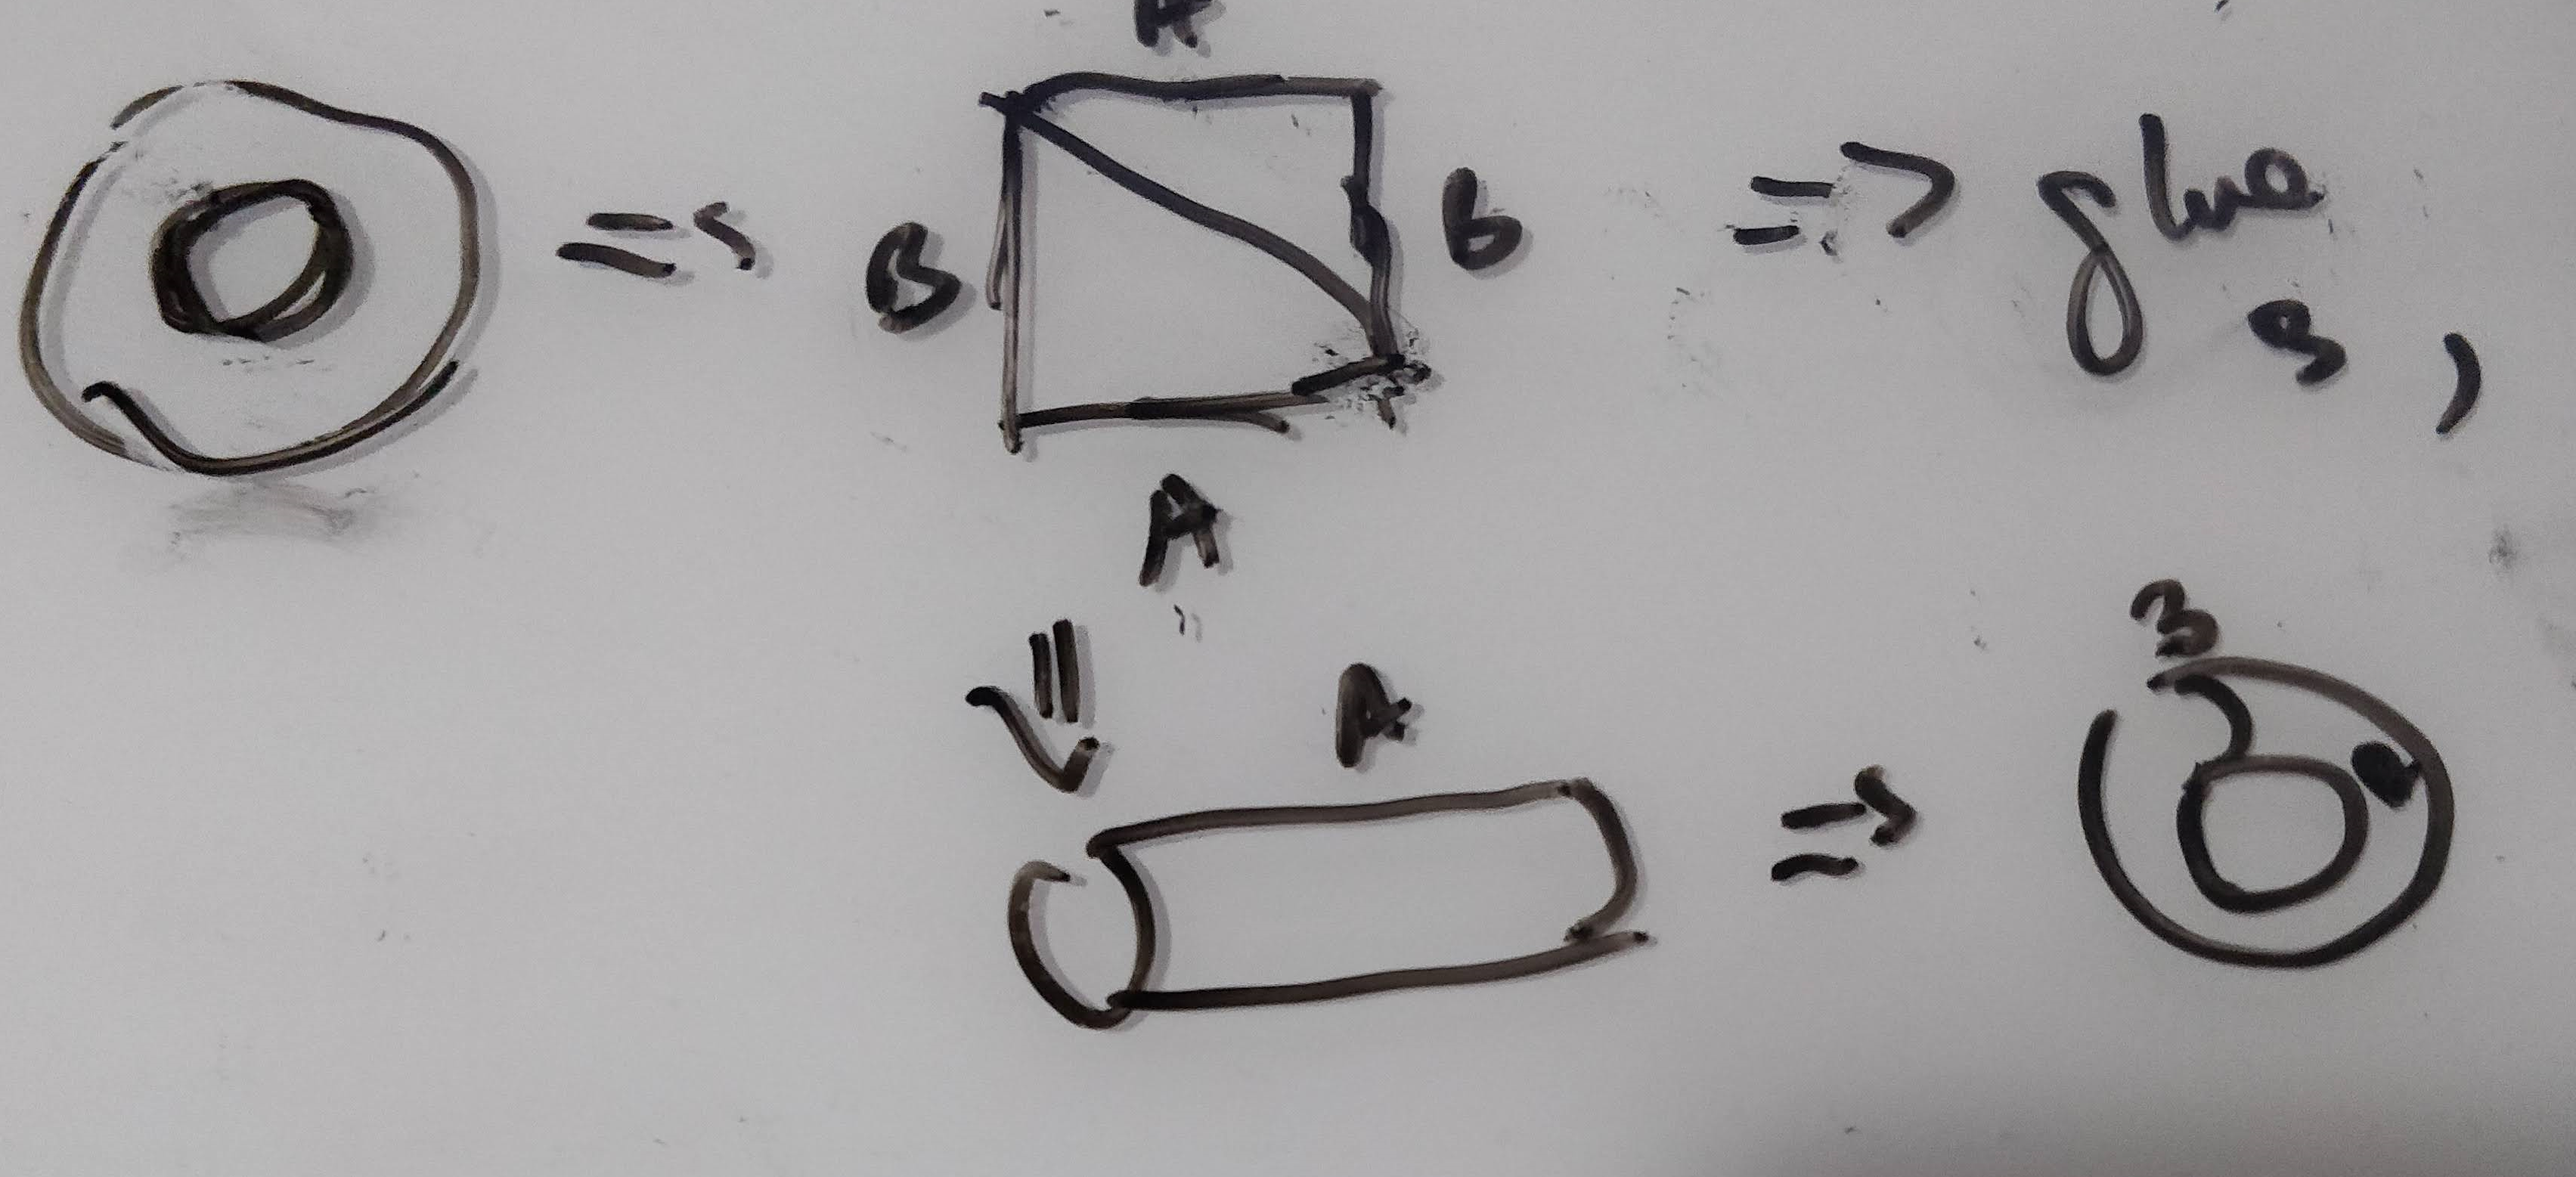
\includegraphics[width=\textwidth]{figures/math/triangle_torus.png}
    \caption{The torus \dtotal is unraveled into a simplacial complex of 2 faces \dbase. Transition functions are defined on the edges of \dbase such that surface can be glued back into the torus.
    \note{add cross sections a and b to ring and color same as edges in complex}}
    \label{fig:triangle_torus}
\end{figure}
An advantage of fiber bundles is the ability to encode data continuity that is more complex than points, a line or a plane. For example, the tori in figure~\ref{fig:triangle_torus} can be unraveled into a simplacial complex of two triangles with labeled edges. Transition functions $\delta$ are defined on the edges such that $a$ can be glued to $a^\prime$ and $b$ to $b^\prime$ to reconstruct the torus. This simplacial complex is then used as the base space encoding the continuity of data that lies in the torus. A constraint on the transition functions is that the monoid actions on the fibers on the edges of \dtotal\ are commutative $\monoid*\dfiber\mapsto \delta(\monoid\dfiber)= \monoid*\delta(\dfiber)$

\begin{figure}[H]
    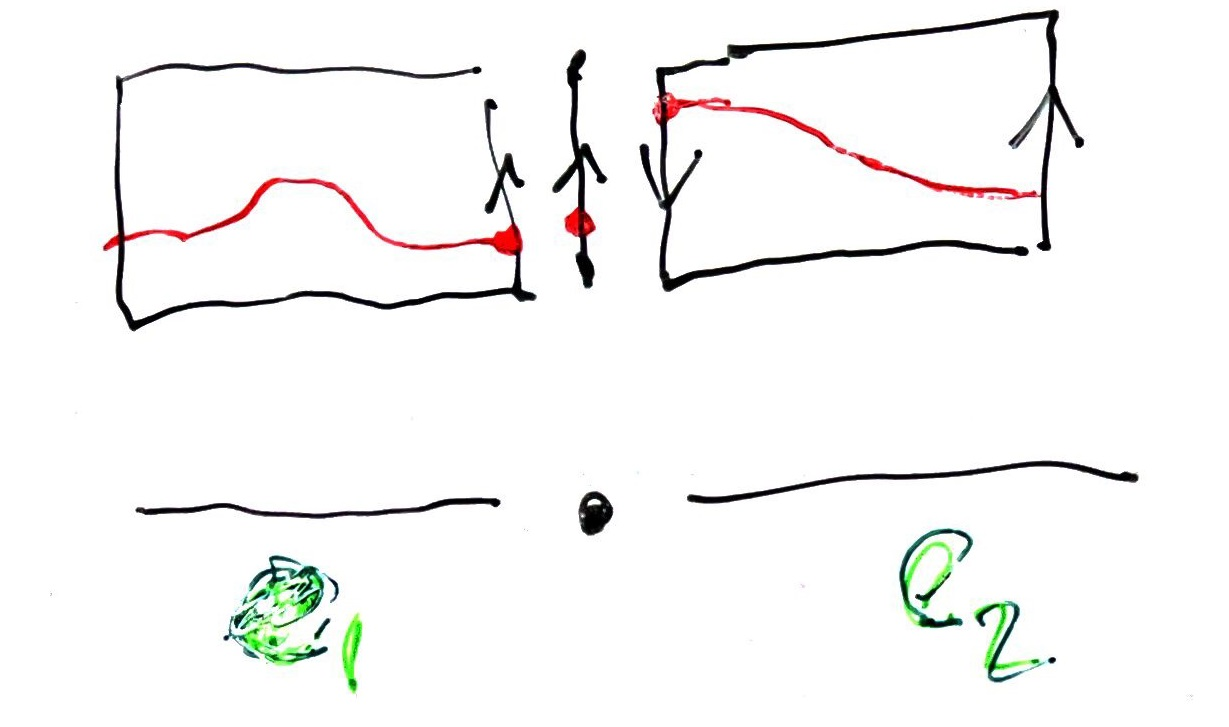
\includegraphics[width=\textwidth]{figures/math/transition_functions.png}
    \caption{Many non-trivial spaces can be made locally trivial by dividing \dtotal into locally trivial subspaces and defining transition functions between the edges on \dbase for how to glue the two subspaces such that the \dsection are continuous.}
    \label{fig:data_base_transition}
\end{figure}
Another advantages of triangulization is that it provides a way to encode non-trivial structures such as the mobius strip\cite{MobiusStripNLab}. As shown in figure ~\ref{fig:data_base_transition}, one way of making the mobius strip trivial is to seperate it into two spaces $\dtotal_1$ and $\dtotal_2$ and then define transition functions that specify that the edges of $\dtotal_1$ need to be reversed to line up with $\dtotal_2$ such that the sections along the edges meet. As with the torus, the transition functions must preserve monoid commutativity. While we generally do not deal with complex or non-trivial bundles, the ability to implement them native to the model allows for a great deal of expressivity in encoding data. This is especially important when developing a tool that needs to be general enough to support any number of very domain specific types of data.